
%(BEGIN_QUESTION)
% Copyright 2011, Tony R. Kuphaldt, released under the Creative Commons Attribution License (v 1.0)
% This means you may do almost anything with this work of mine, so long as you give me proper credit

The compressor automatically shut down last night, tripped by LSHH-231.  The control system alarm log showed a high level alarm LIR-92 about 15 minutes prior to the shutdown:

$$\includegraphics[width=15.5cm]{i0003rx01.eps}$$

Identify the likelihood of each specified fault in this process.  Consider each fault one at a time (i.e. no coincidental faults), determining whether or not each fault could independently account for {\it all} measurements and symptoms in this process.

% No blank lines allowed between lines of an \halign structure!
% I use comments (%) instead, so that TeX doesn't choke.

$$\vbox{\offinterlineskip
\halign{\strut
\vrule \quad\hfil # \ \hfil & 
\vrule \quad\hfil # \ \hfil & 
\vrule \quad\hfil # \ \hfil \vrule \cr
\noalign{\hrule}
%
% First row
{\bf Fault} & {\bf Possible} & {\bf Impossible} \cr
%
\noalign{\hrule}
%
% Another row
2-inch line plugged at bottom of separator vessel &  &  \cr
%
\noalign{\hrule}
%
% Another row
LT-92 failed with high output signal &  &  \cr
%
\noalign{\hrule}
%
% Another row
Air supply to solenoid valve shut off &  &  \cr
%
\noalign{\hrule}
%
% Another row
Solenoid vent line plugged &  &  \cr
%
\noalign{\hrule}
%
% Another row
PSV-11 stuck open &  &  \cr
%
\noalign{\hrule}
%
% Another row
LSHH-231 failed with high output signal &  &  \cr
%
\noalign{\hrule}
} % End of \halign 
}$$ % End of \vbox

Finally, identify the {\it next} diagnostic test or measurement you would make on this system.  Explain how the result(s) of this next test or measurement help further identify the location and/or nature of the fault.

\underbar{file i03475}
%(END_QUESTION)





%(BEGIN_ANSWER)

% No blank lines allowed between lines of an \halign structure!
% I use comments (%) instead, so that TeX doesn't choke.

$$\vbox{\offinterlineskip
\halign{\strut
\vrule \quad\hfil # \ \hfil & 
\vrule \quad\hfil # \ \hfil & 
\vrule \quad\hfil # \ \hfil \vrule \cr
\noalign{\hrule}
%
% First row
{\bf Fault} & {\bf Possible} & {\bf Impossible} \cr
%
\noalign{\hrule}
%
% Another row
2-inch line plugged at bottom of separator vessel & $\surd$ &  \cr
%
\noalign{\hrule}
%
% Another row
LT-92 failed with high output signal &  & $\surd$ \cr
%
\noalign{\hrule}
%
% Another row
Air supply to solenoid valve shut off & $\surd$ &  \cr
%
\noalign{\hrule}
%
% Another row
Solenoid vent line plugged &  & $\surd$ \cr
%
\noalign{\hrule}
%
% Another row
PSV-11 stuck open &  & $\surd$ \cr
%
\noalign{\hrule}
%
% Another row
LSHH-231 failed with high output signal &  & $\surd$ \cr
%
\noalign{\hrule}
} % End of \halign 
}$$ % End of \vbox


%(END_ANSWER)





%(BEGIN_NOTES)

From all the evidence, it seems we really had a high-high level condition in the separator boot, and that the shutdown system acted precisely as it was designed to do: protect the compressor from sucking in any liquid.

\vskip 10pt

A good ``next test'' to do would be to place controller LIC-92 in manual mode and attempt to cycle control valve LV-92, while monitoring solenoid valve SV-92.  If these valves function as they should, the problem may be an obstruction in the drain line.  If they do not function as they should, the problem is either in one of those valves or in the wiring/tubing connecting those valves to the rest of the system.





\vskip 20pt \vbox{\hrule \hbox{\strut \vrule{} {\bf Virtual Troubleshooting} \vrule} \hrule}

This question is a good candidate for a ``Virtual Troubleshooting'' exercise.  Presenting the diagram to students, you first imagine in your own mind a particular fault in the system.  Then, you present one or more symptoms of that fault (something noticeable by an operator or other user of the system).  Students then propose various diagnostic tests to perform on this system to identify the nature and location of the fault, as though they were technicians trying to troubleshoot the problem.  Your job is to tell them what the result(s) would be for each of the proposed diagnostic tests, documenting those results where all the students can see.

During and after the exercise, it is good to ask students follow-up questions such as:

\begin{itemize}
\item{} What does the result of the last diagnostic test tell you about the fault?
\item{} Suppose the results of the last diagnostic test were different.  What then would that result tell you about the fault?
\item{} Is the last diagnostic test the best one we could do?
\item{} What would be the ideal order of tests, to diagnose the problem in as few steps as possible?
\end{itemize}

%INDEX% Basics, control loop troubleshooting
%INDEX% Measurement, pressure: troubleshooting
%INDEX% Process: gas compressor inlet separator (realistic P&ID shown)

%(END_NOTES)

